\chapter{Noci'on de Probabilidades}

\section{Introducci'on}

Al intentar repetir una misma medici'on, los resultados obtenidos no son exactamente iguales debido a peque\~nas variaciones en las variables que no est'an totalmente controladas. Otra posible fuente de error, podr'ia ser el instrumento de medici'on, ya que 'este puede sufrir peque\~nas variaciones para una misma medici'on. En consecuencia, se dice que dicho experimento tiene una \textbf{componente aleatoria}.	
	
	En algunos casos, las variaciones son tan peque\~nas que podr'ian ignorarse. Sin embargo, en general la componente aleatoria s'i est'a presente y su magnitud puede ser muy importante para obtener alguna conclusi'on. Por lo tanto, lo que buscamos es describir, cuantificar y modelar este tipo de variaciones.

En la figura \ref{fig-sistema-modelo} se muestra el esquema idealizado de un experimento, donde el resultado de un experimento depende s'olo del sistema f'isico bajo estudio y de los par'ametros iniciales del experimento.
\begin{figure}[h!]
\begin{center}
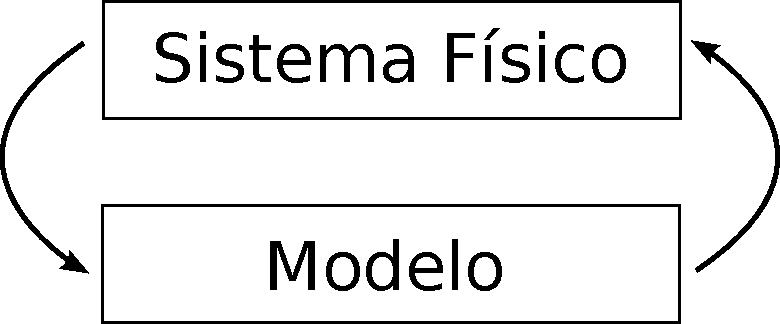
\includegraphics[width=6cm]{figs/fig-sistema-modelo.pdf}
\caption{Sistema f'isico y modelo.}
\end{center}
\label{fig-sistema-modelo}
\end{figure}
 Sin embargo, en la pr'actica siempre existen variables no controladas que pueden influir en el resultado (y/o puede ocurrir que el sistema bajo estudio presente propiedades intrinsecamente aleatorias, como ocurre con distintos sistemas con propiedades cu'anticas), por lo que un esquema un poco m'as realista ser'ia el que se muestra en la figura \ref{fig-entrada-sistema-salida-variables}.
\begin{figure}[h!]
\begin{center}

\includegraphics[width=10cm]{figs/fig-entrada-sistema-salida.pdf}
\caption{Entrada, sistema y salida.}
\end{center}
\label{fig-entrada-sistema-salida}
\end{figure}	
\begin{figure}[h!]
\begin{center}
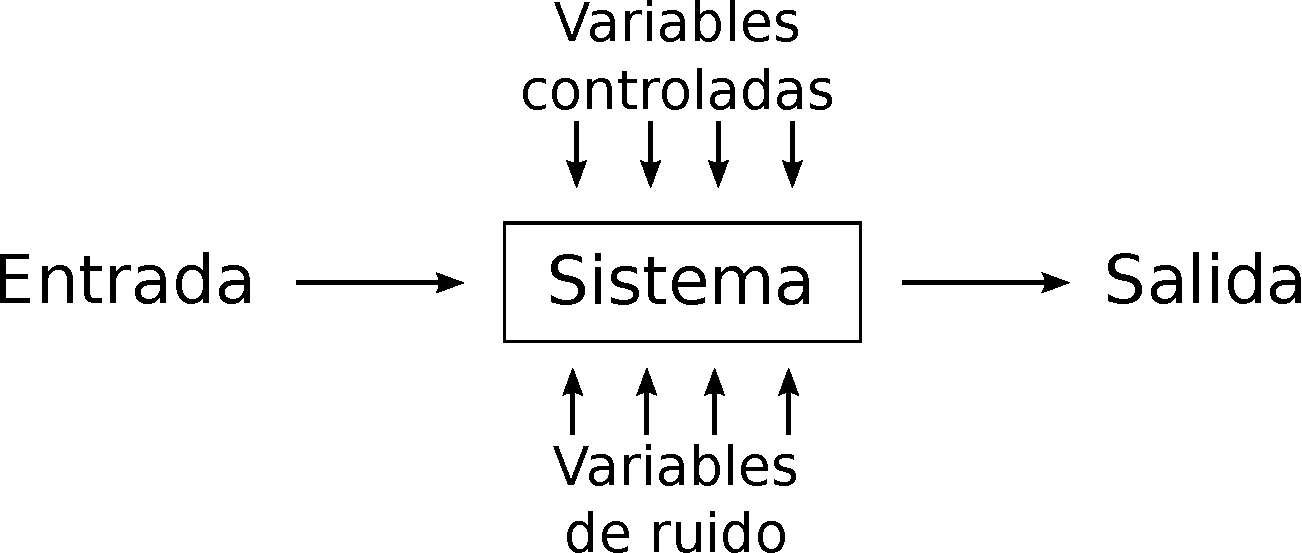
\includegraphics[width=10cm]{figs/fig-entrada-sistema-salida-variables.pdf}
\caption{Entrada, sistema, salida y variables.}
\end{center}
\label{fig-entrada-sistema-salida-variables}
\end{figure}

A continuaci'on introduciremos algunos conceptos b'asicos que resultan 'utiles en la definici'on y discusi'on de probabilidades.
		
\subsection{Experimento aleatorio}

Un \textbf{experimento aleatorio} es aquel que proporciona diferentes resultados a'un cuando se repita siempre de la ``misma manera''. Esto puedo ocurrir ya sea porque existen variables no  controladas o desconocidas que influyen y modifican el resultado, o bien porque el fen'omeno estudiado es intr'insicamente aleatorio.

\subsection{Poblaci'on}
La \textbf{poblaci'on} es un conjunto de elementos (individuos, objetos, etc.) con alguna caracter'istica com'un observable. A los elementos que conforman la poblaci'on se les llama \textbf{unidad observable} o \textbf{unidad de observaci'on}. Cuando se posee informaci'on de todas las unidades observables de la poblaci'on se est'a en presencia de un \textbf{censo}.

%\subsection{Muestra}
%Parte o porci'on extra'ida de una poblaci'on por m'etodos que permitan considerarla como representativa de la misma.


\subsection{Espacio muestral}

El conjunto de los posibles resultados de un experimento aleatorio recibe el nombre de \textbf{espacio muestral} del experimento. El espacio muestral se denotar'a con la letra $S$. Un espacio muestral es \textbf{discreto} si est'a formado por un conjunto de resultados contables.

\subsection{Evento}
Un evento es un subconjunto de un espacio muestral de un experimento aleatorio.
Dos eventos, $E_1$ y $E_2$, tales que $E_1\cap E_2=\emptyset$, se dice que son \textbf{mutuamente excluyentes}. Decimos que $X_i$ ($i=1,2,\cdots$) son \textbf{eventos elementales} si son mutuamente excluyentes ($X_i\cap X_j=\emptyset$, para $i\neq j$) y adem'as $\cup_i X_i=S$. En otras palabras, los eventos $X_i$ son tales que la ocurrencia de uno implica que ninguno de los otros eventos ocurre, y que cualquier otro evento no-elemental puede entenderse como la ocurrencia simult'anea de ellos.

\paragraph{Ejemplo 1:} Considere un experimento en el cual se miden dos variables y 'estas pueden tomar dos valores, $a$ o $b$. Los posibles resultados de dicho experimento ser'an:                                       $S=\{aa,ab,ba,bb\}$ y posibles eventos ser'an $E_1=\{aa\}$, $E_2=\{ab,ba\}$, $E_3=\{aa,ab,ba\}$, $E_4=\{ab,ba,bb\}$, $E_5=\{bb\}$.
		 
\paragraph{Ejemplo 2:} Supongamos que tenemos tres objetos $(1, 2, 3)$ y sacamos un par de 'estos. Todos los posibles resultados ser'an:
\begin{align}
S_1 &= \{12,13,21,23,31,32\}, \\
S_2 &= \{11,12,13,21,22,23,31,32,33\},
\end{align}
dependiendo si una vez sacado cada objeto, 'este es o no remplazado.
		 
\section{Interpretaci'on de la Probabilidad}

Es 'util cuantificar la posibilidad que se presente un resultado de un experimento aleatorio. La posibilidad de un resultado se cuantifica asign'andole un n'umero real en el intervalo $[0,1]$ o un porcentaje entre $0$ y $100\%$. Mientras m'as grande sea el n'umero, mayor ser'a la probabilidad de obtener ese resultado.

Una posible interpretaci'on de la probabilidad\footnote{Esta es la \textbf{interpretaci'on frecuentista}. En F'isica tambi'en es usada la \textbf{interpretaci'on Bayesiana}, que no discutiremos en mayor detalle en este curso.} se basa en el modelo de la \textit{repetici'on del experimento aleatorio}.
Sea $n(E)$ el n'umero de veces que ocurre el evento $E$ y $N$ el n'umero de veces que se realiza el experimento. Es intuitivamente razonable tomar como valor de $P(E)$ a
\begin{equation}
P(E):=\lim_{N\to\infty}f(E)=\lim_{N\to\infty}\frac{n(E)}{N},
\end{equation}
es decir, como el valor l'imite de la fracci'on de veces que el resultado $E$ aparece en $N$ repeticiones del experimento aleatorio, a medida que $N$ crece sin cota alguna. 

Por ejemplo, cada vez que un espacio muestral est'a formado por $d$ posibles resultados \textit{igualmente probables}, la probabilidad de cada uno de ellos ser'a $1/d$.

%Para un espacio muestral discreto, la probabilidad de un evento $E$, denotada como $P(E)$, es igual a la suma de las probabilidades de los resultados en $E$.
		
\section{Axiomas de probabilidad}

La probabilidad es un n'umero que se asigna a cada miembro de una colecci'on de eventos de un experimento aleatorio y que satisface las siguientes propiedades.

\begin{itemize}
\item Si $S$ es el espacio muestral y $E$ es cualquier evento del experimento aleatorio,
\begin{equation}
P(S)=1,\qquad 0\le P(E)\le 1.
\end{equation}
\item Si $E_1$ y $E_2$ son eventos excluyentes, es decir, $E_1\cap E_2=\emptyset$, entonces
\begin{equation}
P(E_1\cup E_2)=P(E_1)+P(E_2).
\end{equation}
\end{itemize}

\subsection{Consecuencias directas de los axiomas}
\begin{itemize}
\item La probabilidad de no obtener ning'un resultado es nula:
\begin{equation}
P(\emptyset)=0.
\end{equation}
\item La probabilidad de obtener el \textbf{evento complementario} $E'$ a un evento $E$:
\begin{equation}
P(E')=1-P(E).
\end{equation}
\item La probabilidad de un evento $E_1$ contenido en otro evento $E_2$, es decir tal que $E_1\subseteq E_2$,  es menor que la probabilidad de $E_2$:
\begin{equation}
P(E_1)\le P(E_2).
\end{equation}
\end{itemize}
\paragraph{Ejemplo:} Considere que el espacio muestral de un experimento aleatorio es dado por $S=\{a,b,c,d,e\}$, donde $a$,\dots,$e$ son eventos elementales con probabilidades $0.1, 0.1, 0.2, 0.4$ y $0.2$ respectivamente. Sean adem'as los eventos $A=\{a,b\}$ ($a$ 'o $b$), $B=\{c,d,e\}$ ($c$ 'o $e$ 'o $e$). Determinar:
\begin{align}
P(A) &= 0.1+0.1, \\
P(B) &= 0.2+0.4+0.2, \\
P(A\cup B) &= 0.1+0.1+0.2+0.4+0.2, \\
P(A\cap B) &= P(\emptyset) = 0.
\end{align}

\section{Reglas de adici'on}

% La probabilidad de un evento compuesto, como  uniones, intersecciones y complementos, a menudo se pueden obtener a partir  de las probabilidades de cada uno de los eventos individuales. 

Considere dos eventos $A$ y $B$ que no necesariamente son mutuamente excluyentes (decir, que $A\cap B\neq\emptyset$ y por tanto en general $P(A\cap B)\neq 0$.). Entonces la probabilidad de obtener $A$ o bien $B$ es dada, ver figura \ref{fig-A-B}, por
\begin{figure}[h!]
\begin{center}
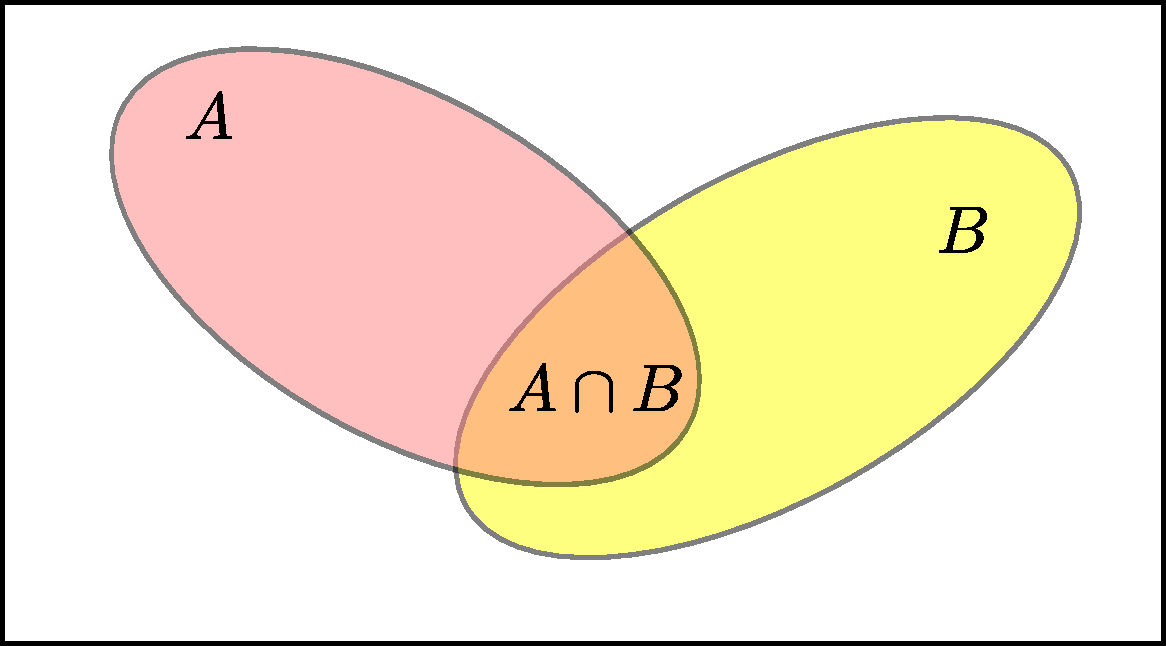
\includegraphics[width=7cm]{figs/fig-Muestra-A-B.pdf}
\caption{Dos conjuntos y su intersecci'on.}
\end{center}
\label{fig-A-B}
\end{figure}
\begin{equation}
P(A\cup B)=P(A)+P(B)-P(A\cap B).
\end{equation}

\paragraph{Ejemplo:} Se realiza un experimento para determinar el valor de dos magnitudes f'isicas. El n'umero de mediciones son 940, las que se distribuyen seg'un la siguiente tabla:
\begin{table}[h!]
\begin{center}
\begin{tabular}{cc|cc}
 & $Y$ & $C$ & $D$ \\ 
$X$ &  &  &  \\ 
\hline 
$A$ &  & 514 & 68 \\ 
$B$ &  & 112 & 246
\end{tabular} 
\caption{Distribuci'on de las 940 mediciones.}
\end{center}
\end{table}

Sean $E_1$ y $E_2$ los eventos definidos por:
\begin{align}
E_1 &= \left\{\text{todos los resultados donde } X=B\right\},\\
E_2 &= \left\{\text{todos los resultados donde } Y=D\right\}.
\end{align}

Calcular la probabilidad de obtener como resultado los siguientes casos:
\begin{equation}
X=B, \quad Y=D, \quad X=B\wedge Y=D, \quad X=B \vee Y=D, \quad X\neq B \vee Y\neq D.
\end{equation}
\begin{equation}
P(E_1)\approx\frac{358}{940}, \qquad P(E_2)\approx\frac{314}{940}, \qquad P(E_1\cap E_2)\approx\frac{246}{940},
\end{equation}
\begin{equation}
P(E_1\cup E_2)\approx\frac{426}{940}, \qquad P((E_1\cup E_2)')\approx\frac{514}{940}, \qquad P((E_1\cap E_2)')\approx\frac{694}{940}.
\end{equation}

Otra manera de resolver el ejercicio:
\begin{equation}
P(E_1\cup E_2)=P(E_1)+P(E_2)-P(E_1\cap E_2)\approx \frac{358}{940}+\frac{314}{940}-\frac{246}{940}=\frac{426}{940},
\end{equation}
\begin{equation}
P((E_1\cup E_2)')=1-P(E_1\cup E_2)\approx 1-\frac{426}{940}=\frac{514}{940}.
\end{equation}
\section{Probabilidad condicional}

En muchas ocasiones la probabilidad de un evento depende de algunas condiciones, como por ejemplo si otro evento a ocurrido (antes o simultaneamente). En estos casos resulta 'util el concepto de \textbf{probabilidad condicional}.

% Algunos fen'omenos tienden a ocurrir en rachas, esto hace que la probabilidad que ocurra un primer evento es menor que la probabilidad que se repita el evento u ocurra inmediatamente otro asociado al primero.
%		    
%\paragraph{Ejemplo:} Un canal de comunicaci'on digital tiene una tasa de error de un bit por cada mil transmitidos, es decir, la probabilidad que ocurra un error es de 1/1000. Aunque los errores son muy escasos, tienden a ocurrir en rachas, por lo que una vez ocurrido un error, la probabilidad que ocurra un segundo error es mayor que 1/1000. 

\paragraph{Definici'on:} La probabilidad condicional de un evento $A$ \textit{dado un evento} $B$, denotada por $P(A|B)$, es 
\begin{equation}\label{PAB}
P(A|B):=\frac{P(A\cap B)}{P(B)},
\end{equation}
de modo que 
\begin{equation}\label{PAyB}
P(A\cap B)=P(A|B)\cdot P(B).
\end{equation}
En palabras: ``la probabilidad de que ocurra $A$ y $B$ es igual a la probabilidad de que ocurra $A$ \underline{\textit{dado}} $B$, multiplicada por la probabilidad de que ocurra $B$".

%Consideremos un caso en que todos los resultados de un experimentos aleatorio son igualmente probables. Si existe un total de $n$ resultados
%\begin{equation}
%P(B)=\frac{(\#\text{ de resultados en }B)}{n},
%\end{equation}
%\begin{equation}
%P(A\cap B)=\frac{(\#\text{ de resultados en }A\cap B)}{n},
%\end{equation}
%\begin{equation}
%\frac{P(A\cap B)}{P(B)}=\frac{(\#\text{ de resultados en }A\cap B)}{(\#\text{ de resultados en }B)} = \text{frecuencias relativas},
%\end{equation}

Decimos que $A$ y $B$ son \textbf{eventos independientes} si se tiene que
\begin{equation}
P(A|B)=P(A), 
\end{equation}
es decir, que el resultado de $B$ no influye en la probabilidad de obtener $A$. En este caso  \eqref{pAyB} implica que
\begin{equation}\label{pAyB}
P(A\cap B)=P(A)\cdot P(B),
\end{equation}
y adem'as que
\begin{equation}
P(B|A)=P(B).
\end{equation}


\begin{figure}[h!]
\begin{center}
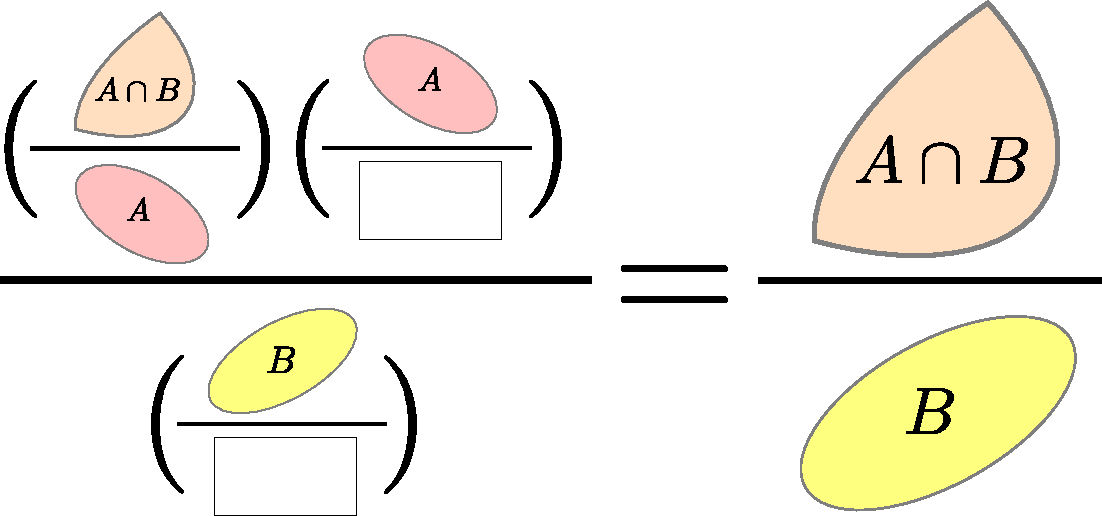
\includegraphics[width=7cm]{figs/fig-P-A-B.pdf}
\caption{Representaci'on diagram'atica de la Probabilidad condicional \eqref{PAB}.}
\end{center}
\label{fig-P-A-B}
\end{figure}
\textbf{Ejemplo:} Suponga que medimos la presencia de los contaminantes $A$ y $B$ en muestras de vino. Medimos 266 muestras de vino, las cuales arrojan el siguiente resultado: 
\begin{table}[h!]
\begin{center}
\begin{tabular}{cc|cc}
 & $A$ & S'i & No \\ 
$B$ &  &  &  \\ 
\hline 
S'i &  & 12 & 18 \\ 
No &  & 24 & 212
\end{tabular} 
\caption{Contaminantes en muestras de vino.}
\end{center}
\end{table}
\begin{equation}
P(B|A)=\frac{P(B\cap A)}{P(A)}\approx\frac{\frac{12}{266}}{\frac{36}{266}}=\frac{12}{36}=\frac{1}{3}\approx 0.33.
\end{equation}
Calculemos $P(A)$ y $P(A|B)$ para construir un diagrama, llamado diagrama 'arbol, y as'i poder comprender mejor lo que est'a pasando.
\begin{figure}[h!]
\begin{center}
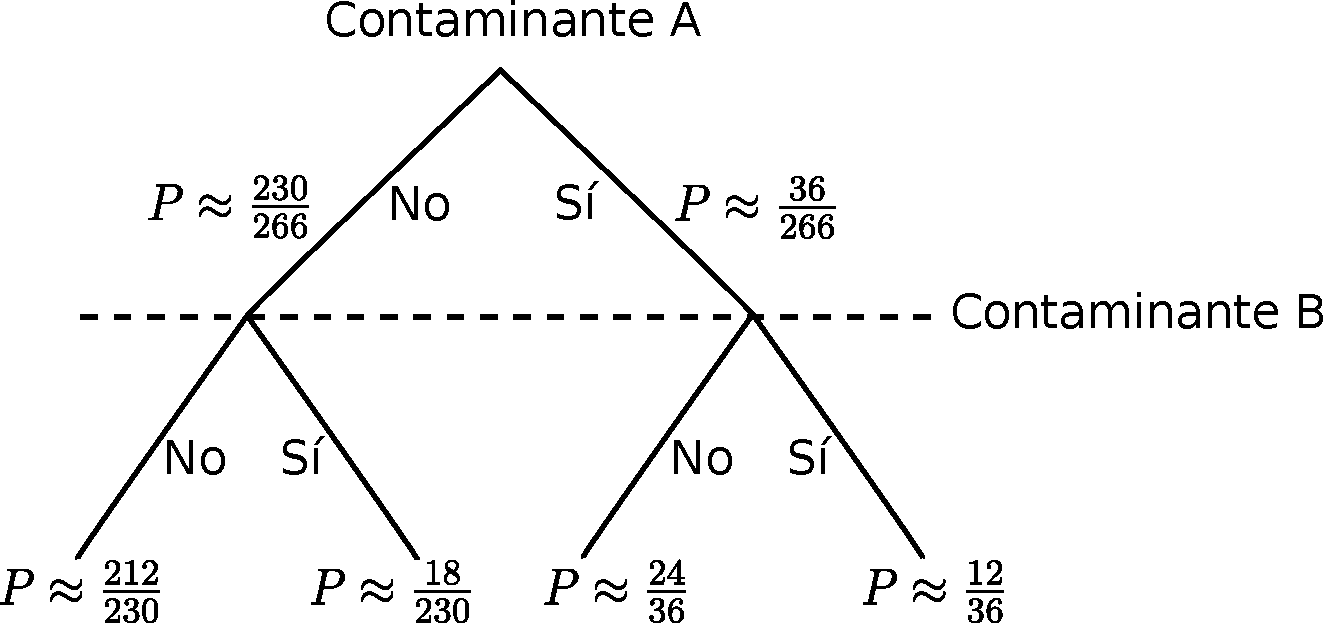
\includegraphics[width=10cm]{figs/fig-arbol.pdf}
\caption{Diagrama 'arbol.}
\end{center}
\label{fig-arbol}
\end{figure}
%Para procesos independientes la probabilidad que ocurra un evento $A$ cuando ya ha ocurrido otro evento $B$ con anterioridad, es simplemente igual a la probabilidad de $A$ (independiente de lo que pase con el evento $B$). 

%\paragraph{Definici'on:} Dos eventos son independientes si, y s'olo si, cualquiera de las proposiciones es verdadera.
%\begin{itemize}
%\item $P(A|B)=P(A)$.
%\item $P(B|A)=P(B)$.
%\item $P(A\cap B)=P(A)P(B)$.
%\end{itemize}




\subsection{Reglas de multiplicaci'on}
Como vimos, la definici'on \eqref{PAB} de probabilidad condicional implica la relaci'on \eqref{PAyB}. Esta regla de multiplicaci'on puede ser extendida a un n'umero finito de eventos ${A_i}$:
\begin{equation}
P({\bigcap^k_{i=1} A_i})=P(A_1)P(A_2|A_1)P(A_3|A_1\cap A_2)\cdots P(A_n|\bigcap^{k-1}_{i=1} A_i).
\end{equation}

\subsection{Reglas de Probabilidad total}

Cualquier evento puede escribirse como la uni'on de la parte de $B$ que se encuentra en $A$ m'as la parte de $B$ que est'a en el complemento de $A$.
(Ver figura)
\begin{equation}
B=(A \cap B) \cup (A'\cap B).
\end{equation}
Note que $(A \cap B)$ y $(A'\cap B)$ son mutuamente excluyentes. Si calculamos la probabilidad del evento $B$ usando la propiedad de uni'on y la regla de multiplicaci'on obtenemos:
\begin{equation}
P(B)=P(A \cap B)+P(B \cap A')=P(B|A)P(A)+P(B|A')P(A').
\end{equation}

\begin{figure}[h!]
\begin{center}
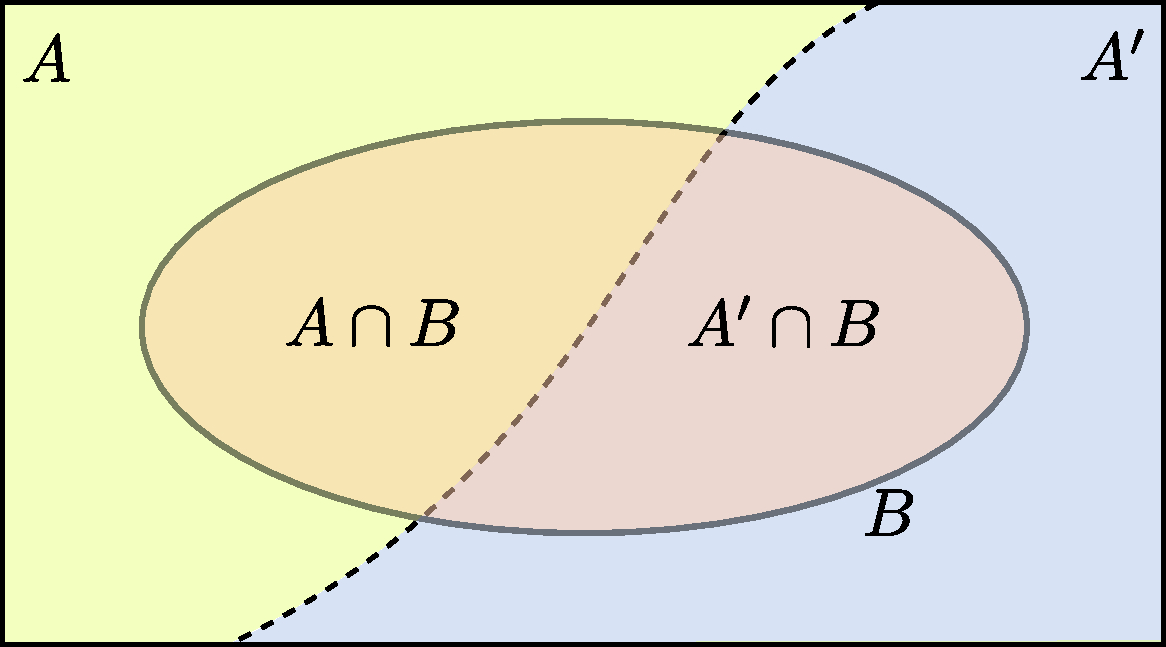
\includegraphics[width=6cm]{figs/fig-conjuntos.pdf}
\caption{Diagrama de Venn para la probabilidad total.}
\end{center}
\label{fig-conjuntos}
\end{figure}

\subsection{Teorema de Bayes}
Retomando la definici'on de probabilidad condicional \eqref{PAB} y las reglas de multiplicaci'on, es directo probar que:
\begin{equation}
P(A|B)=\frac{P(B|A)P(A)}{P(B)}.
\end{equation}
Este resultado es de gran utilidad ya que permite determinar $P(A|B)$ en funci'on de $P(B|A)$.


\textbf{Ejemplo:} Supongamos que mediante un an'alisis de 84 muestras se detectan 36 muestras con Pb, 28 con As, 12 con ambos elementos pesados y 32 est'an libres de contaminaci'on. Calcular la probabilidad de encontrar Pb entre las muestras que presentaron As: $P(\text{Pb}|\text{As})$.

\begin{table}[h!]
\begin{center}
\begin{tabular}{cc|cc}
& Pb & No & S'i \\ 
As & & & \\
\hline 
No & & 32 & 24 \\ 
S'i & & 16 & 12
\end{tabular} 
\caption{Pb y As en 84 muestras de vino.}
\end{center}
\end{table}

Usando el teorema de Bayes tenemos que
\begin{equation}
P(\text{Pb}|\text{As})= \frac{P(\text{As}|\text{Pb})P(\text{Pb})}{P(\text{As})},
\end{equation}
\begin{equation}
P(\text{Pb}|\text{As})\approx \frac{\frac{12}{36} \frac{36}{84}}{\frac{28}{84}}=\frac{12}{28}= \frac{3}{7}\approx 0.43.
\end{equation}
%Si se conocen los siguientes datos $P(\text{As}|\text{Pb})\approx 0.33$, $P(\text{Pb})\approx 0.43$, $P(\text{As})\approx 0.33$, calcular $P(\text{Pb}|\text{As})$. Usando el teorema de Bayes el c'alculo es muy simple, 
%\begin{equation}
%P(\text{Pb}|\text{As})\approx \frac{0.33 \times 0.43}{0.33}=0.43.
%\end{equation}




\section{Variables aleatorias}

\paragraph{Definici'on:} Sea $S=\{s_1,s_2,\dots,s_D\}$ un espacio muestral, cuyos elementos $s_\alpha$ ($\alpha=1,\cdots,D$) representan los posibles resultados distintos de un experimento aleatorio. Sea $X$  una funci'on de valor real definida sobre $S$, de manera que asocie los resultados de $S$ a valores reales. Se dice entonces que $X$ es una \textbf{variable aleatoria} definida sobre el espacio muestral. Entonces $S$ es el dominio de la variable aleatorio $X$ y el rango de esta funci'on es el conjunto de valores reales $\{x_\alpha=X(s_\alpha)\}$.

Decimos que la variable $X$ es \textbf{discreta} si su rango es un conjunto discreto (finito o infinito numerable) de n'umeros reales, en caso contrario decimos que $x$ es una variable \textbf{continua}.

\begin{figure}[h!]
\begin{center}
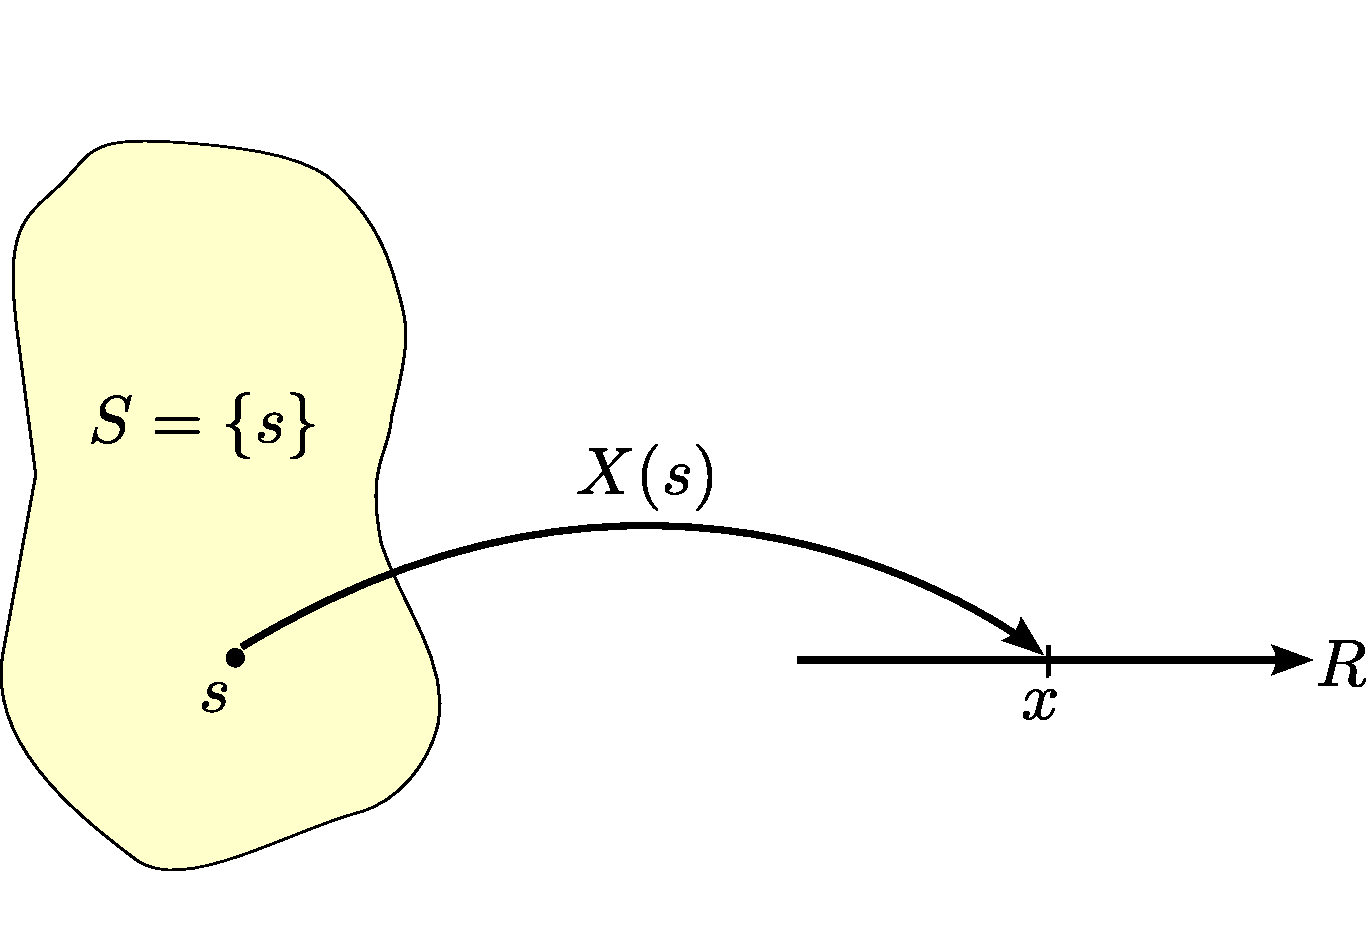
\includegraphics[width=6cm]{figs/fig-esp-muestral.pdf}
\caption{Espacio Muestral, funci'on aleatoria y rango.}
\end{center}
\label{fig-esp-muestral}
\end{figure}

Denotaremos al conjunto de todos los \textit{valores distintos} de $\{x_\alpha\}$ por $\{x_a\}$, con $a=1,\cdots, d$. Note que, si la funci'on aleatoria asigna el mismo valor real a al menos dos elementos del espacio muestral, entonces $d\le D$.

\section{Histogramas}

Luego de realizar un experimento aleatorio, se tiene un conjunto de resultados. 
%Se busca una forma de representar apropiadamente c'omo se distribuyen estas medidas.
%La idea es presentar los resultados de la mejor forma posible para poder tener una idea de como se distribuyen los datos en funcion de todos los valores distintos que puede tomar la variable aleatoria. 
Una de las mejores maneras de representar gr'aficamente la distribuci'on de los resultados es construir un \textbf{histograma}, es decir, un gr'afico de frecuencias (o n'umero de ocurrencias) para cada valor distinto de la variable aleatoria (los $\{x_a\}$).

 Como primer paso se divide el conjunto de valores de la variable aleatoria en un cierto n'umero de intervalos (intervalos de clase o celdas). Luego se grafica en el eje de las ordenadas los intervalos de clase y en el eje de las abscisas el número de veces que los resultados están contenidos en cada uno de los respectivos intervalos. Otra forma de representar los resultados es mediante un gr'afico de \textbf{frecuencias relativas}, que se diferencia del anterior en que en el eje de las abscisas ahora se grafica las frecuencias divididas por el n'umero total de datos.
%  De esta manera las frecuencias relativas son la probabilidad que la variable aleatoria tome cierto valor \textit{en la muestra} (y que se espera que sea un buen estimador de la probabilidad de la poblaci'on).

\paragraph{Ejemplo:} Arrojemos dos dados y para cada lanzamiento sumemos las dos caras superiores. Luego de repetir este experimento 100.000 veces, construyamos un histograma y un gr'afico de frecuencias relativas a partir de los datos experimentales. En este caso el gr'afico de frecuencias relativas nos permite estimar c'omo es la distribución de probabilidades de la variable aleatoria.
\begin{table}[h!]
\begin{center}
\begin{tabular}{c|c|c|c|c|c|c|c|c|c|c|c}
$x_\alpha$ & 2 & 3 & 4 & 5 & 6 & 7 & 8 & 9 & 10 & 11 & 12 \\ \hline
$n_\alpha$ & 2703 & 5526 & 8320 & 11205 & 13685 & 16778 & 13870 & 11173 & 8517 & 5511 & 2712
\end{tabular} 
\caption{N'umero de ocurrencias de cada valor de la suma de dos dados. Experimento (simulado) con $10^5$ repeticiones.}
\label{tab-suma-1E5}
\end{center}
\end{table}
\begin{figure}[h!]
\begin{center}
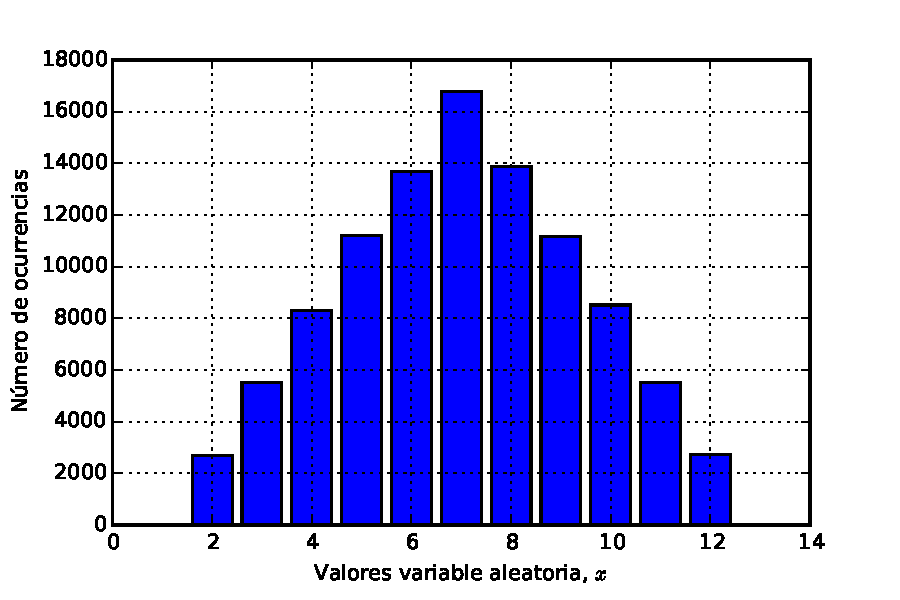
\includegraphics[width=9cm]{figs/fig-barras-dados-1E5.pdf}
\caption{Histograma de valores de suma de dados, de acuerdo a los datos en la tabla \ref{tab-suma-1E5}. C'odigo Python \href{https://github.com/gfrubi/Lab/blob/master/python/fig-conteo-suma-dados.py}{aqu\'i}.}
\end{center}
\label{fig-his-dados-1E5}
\end{figure}
\begin{figure}[h!]
\begin{center}
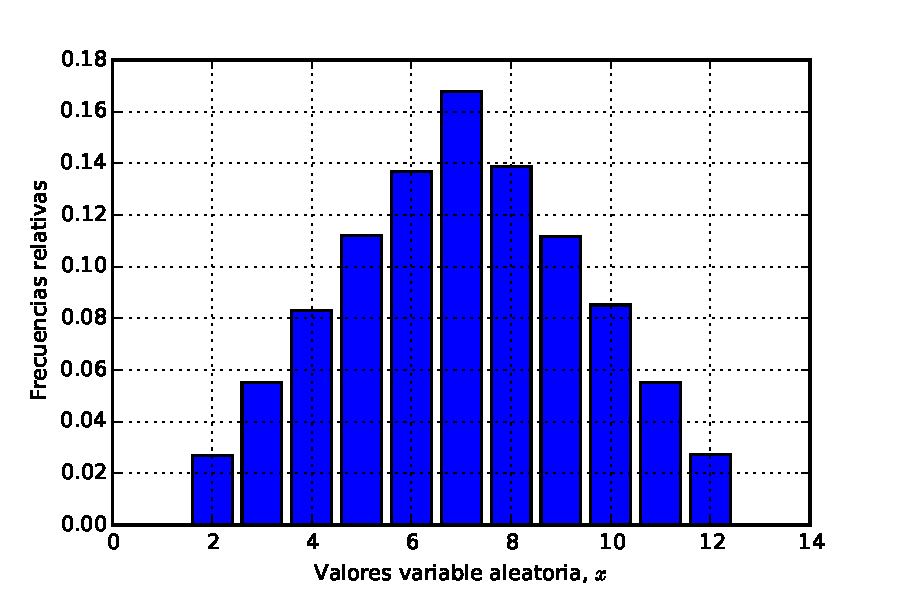
\includegraphics[width=9cm]{figs/fig-frec-relativas-dados-1E5.pdf}
\caption{Frecuencias relativas de ocurrencia de los valores de suma de dados.  C'odigo Python \href{https://github.com/gfrubi/Lab/blob/master/python/fig-frec-relativas-suma-dados.py}{aqu\'i}.}
\end{center}
\label{fig-frec-relativas-dados-1E5}
\end{figure}


\section{Distribuciones de probabilidad}
		 
 Ahora consideraremos un \textit{modelo idealizado} del experimento de los dados (de 6 caras, no cargados). Considere todos los posibles resultados al lanzar estos dos dados. Luego, definamos nuestra variable aleatoria como la suma de las caras de ambos dados, despu'es de ser arrojados. Para este caso el espacio muestral est'a formado por los $D=36$ posibles resultados, \textit{que supondremos igualmente probables}, y para los cuales la variable aleatoria puede tomar $d=11$ valores distintos. Adem'as, existe un cierto n'umero de combinaciones distintas de los resultados de cada dado que generan el mismo valor de la variable aleatoria (la suma), como se muestra en la Tabla \ref{tab-e-m}. Podemos construir un gr'afico de barras del n'umero de combinaciones en funci'on de los valores que toma la variable aleatoria. En este ejemplo, ver figura \ref{fig-bem}, el gr'afico muestra la distribuci'on de combinaciones asociadas a la variable aleatoria. M'as a'un, normalizando este gr'afico respecto al n'umero total de combinaciones (36 en este ejemplo), encontramos un gr'afico de la \textbf{distribuci'on de probabilidad} asociada a cada uno de los posibles valores de la variable aleatoria. Ver figura \ref{fig-probabilidad-dados}.
\begin{table}[h!]
\begin{center}
\begin{tabular}{|c|c|c|}
\hline 
Espacio muestral, $S$ & Valor de la variable & n'umero de  \\ 
(resultados posibles) & aleatoria, $X$ & combinaciones \\ \hline 
$(1,1)$ & 2 & 1 \\ \hline 
$(1,2)$, $(2,1)$ & 3 & 2 \\ \hline 
$(1,3)$,$(2,2)$,$(3,1)$ & 4 & 3 \\ \hline 
$(1,4)$, $(2,3)$, $(3,2)$,$(4,1)$ & 5 & 4 \\ \hline 
$(1,5)$, $(2,4)$, $(3,3)$, $(4,2)$,$(5,1)$ & 6 & 5 \\ \hline 
$(1,6)$,$(2,5)$,$(3,4)$,$(4,3)$,$(5,2)$,$(6,1)$ & 7 & 6 \\ \hline 
$(2,6)$,$(3,5)$,$(4,4)$,$(5,3)$,$(6,2)$ & 8 & 5 \\ \hline 
$(3,6)$,$(4,5)$,$(5,4)$,$(6,3)$ & 9 & 4 \\ \hline 
$(4,6)$,$(5,5)$,$(6,4)$ & 10 & 3 \\ \hline 
$(5,6)$,$(6,5)$ & 11 & 2 \\ \hline 
$(6,6)$ & 12 & 1 \\ \hline 
\end{tabular} 
\caption{N'umero de combinaciones correspondientes a cada valor de la suma de dos dados. En este caso $d=11$.}
\label{tab-e-m}
\end{center}
\end{table}
\begin{figure}[h!]
\begin{center}
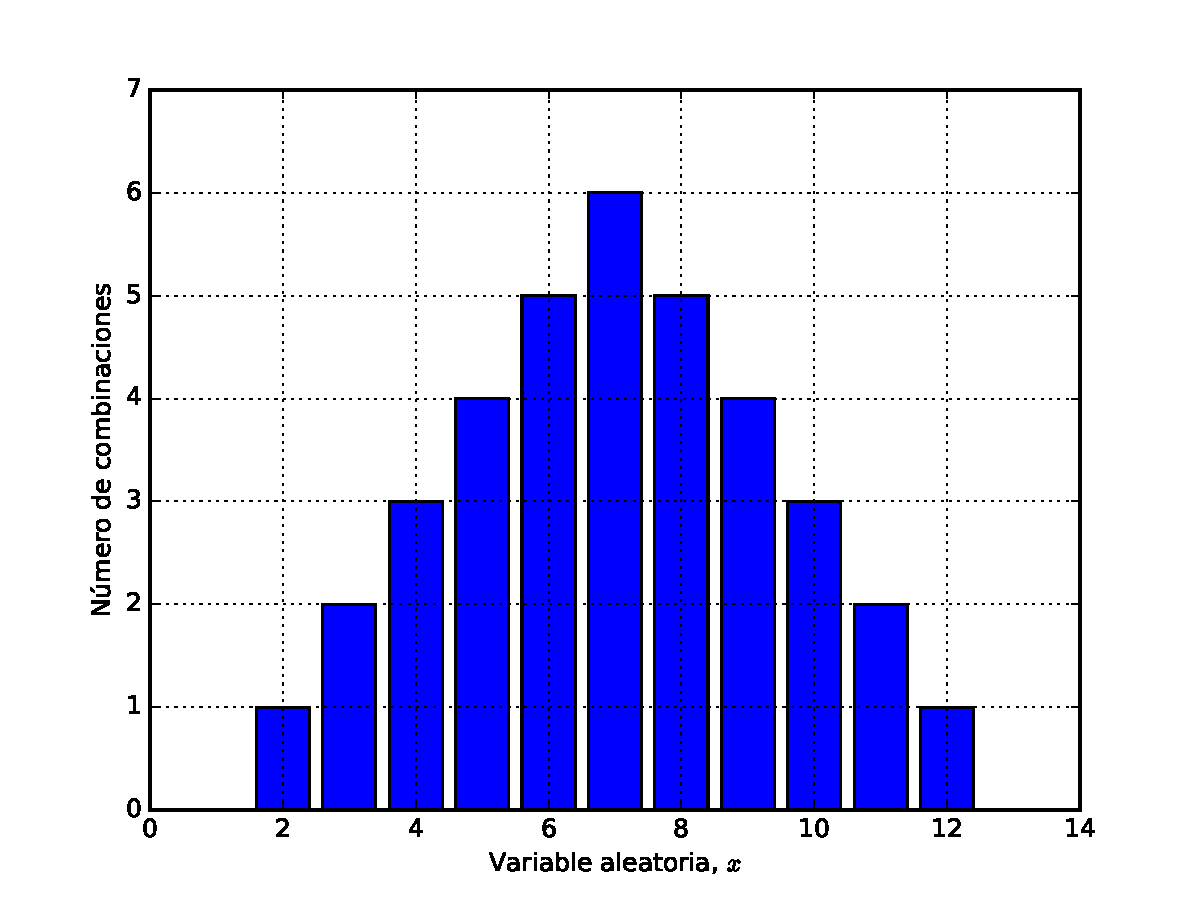
\includegraphics[width=9cm]{figs/fig-combinaciones-suma-dados.pdf}
\caption{Gr'afico de barras para los valores $x$ de la variable aleatoria, de acuerdo a los datos en la tabla \ref{tab-e-m}. C'odigo Python \href{https://github.com/gfrubi/Lab/blob/master/python/fig-combinaciones-suma-dados.py}{aqu\'i}.}
\end{center}
\label{fig-bem}
\end{figure}


\begin{figure}[h!]
\begin{center}
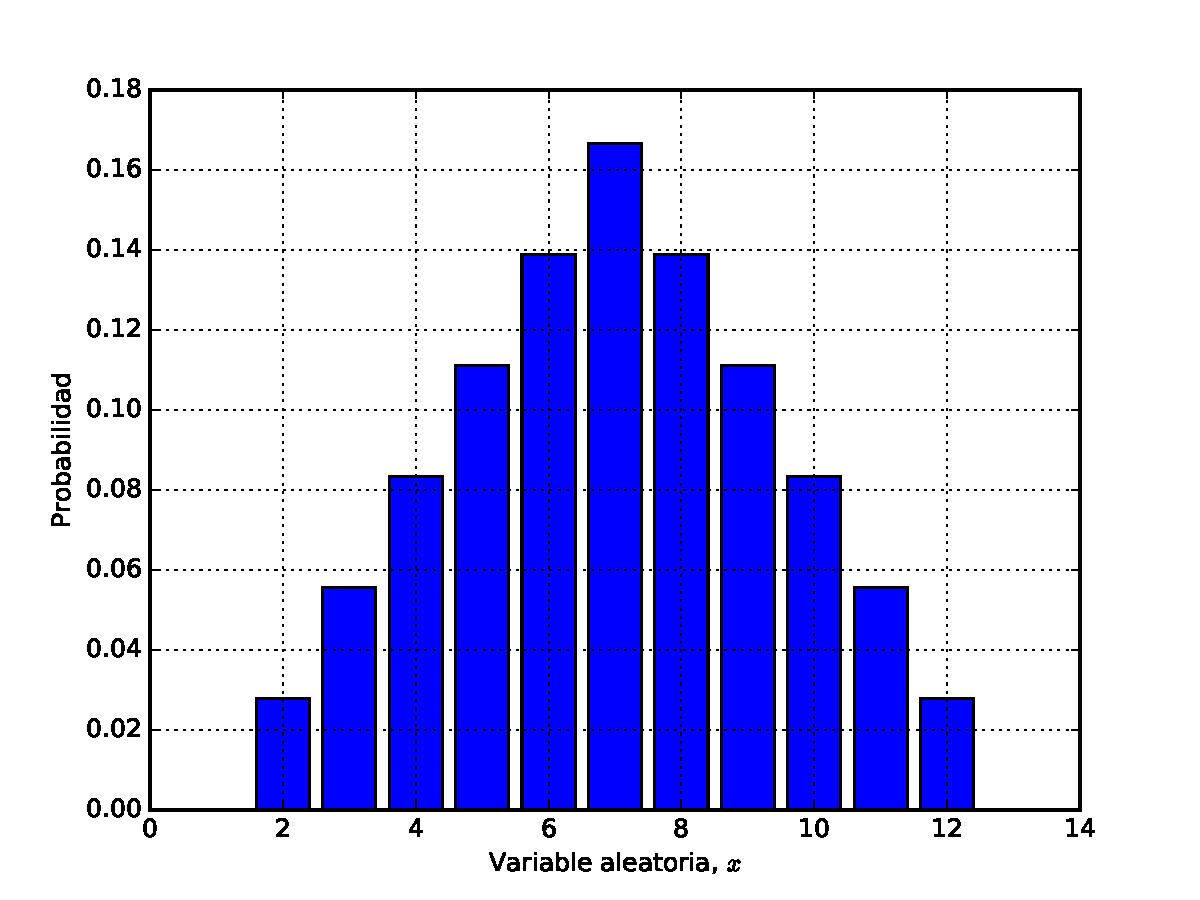
\includegraphics[width=9cm]{figs/fig-probabilidad-suma-dados.pdf}
\caption{Probabilidad para las sumas de las dos caras de dos dados. C'odigo Python \href{https://github.com/gfrubi/Lab/blob/master/python/fig-probabilidad-suma-dados.py}{aqu\'i}.}
\end{center}
\label{fig-probabilidad-dados}
\end{figure}


 Como se desprende del ejemplo, si la variable aleatoria est'a claramente definida, es posible definir una funci'on que asigne una probabilidad que dicha variable tome un determinado valor. En este caso, esta probabilidad es proporcional al n'umero de combinaciones del espacio muestral asociados a un mismo valor de la variable aleatoria. La mencionada funci'on recibe el nombre de \textbf{funci'on distribuci'on de probabilidad} de la variable aleatoria $X$. El t'ermino m'as general, \textbf{distribuci'on de probabilidad}, se refiere no s'olo a la funci'on de probabilidad, sino tambi'en a la \textbf{funci'on de distribuci'on acumulativa} de $X$, que definiremos m'as adelante.


%\paragraph{Definici'on:} Llamamos \textbf{evento} ($E$, $E\subseteq S$) a un conjunto de posibles resultados de un experimento aleatorio (Por ejemplo, el evento $E$ puede ser el conjunto de todos los resultados tales que la variable aleatoria sea par). Denotamos por $P(E)$ a la probabilidad de ocurrencia de este evento. (En nuestro ejemplo, $P(E)=P(x=2)+P(x=4)+P(x=6)+\cdots +P(x=12)$).


\paragraph{Definici'on:} La \textbf{funci'on de probabilidades} $p_X$ para una variable aleatoria discreta $X$ est'a definida como el conjunto $p_X=\{p_a\}$ de todas las probabilidades de ocurrencia de cada valor posible $x_a$ de la variable aleatoria, con
\begin{equation}
p_a=P(X=x_a) , \qquad   a=1,\cdots, d,
\end{equation}
y debe satisfacer las siguientes condiciones:
\begin{equation}
p_a\geq 0, \qquad  a=1,\cdots, d,
\end{equation}
\begin{equation}
\sum_{a=1}^d p_a=1.
\end{equation}
		 
\paragraph{Definici'on:} La \textbf{funci'on de distribuci'on acumulativa} (``cumulative distribution function'', cdf) de una variable aleatoria discreta $X$, es la probabilidad que el valor de $X$ sea menor o igual a un valor especifico $x$ y est'a dado por:
\begin{equation}
F_X(x)=P(X\le x)=\sum_{x_a\le x}p_X(x_a)=\sum_{x_a\le x}p_a.
\end{equation}
		
Como consecuencia, la probabilidad de que la variable $X$ \textit{adopte un valor mayor que $x$} es
\begin{equation}
P(X> x) = 1 - F_X(x),
\end{equation}
y la probabilidad de que la variable $X$ \textit{adopte un valor mayor que $a$ y menor o igual a $b$}, es decir, en el intervalo $(a,b]$ es
\begin{equation}
P(a<X\le b) = F_X(b)-F_X(a).
\end{equation}
%	Por lo tanto, en el caso discreto, una variable aleatoria est'a caracterizada por la funci'on de probabilidad $p_a$, la cual determina la probabilidad puntual que $X = x_a$ , y por la funci'on distribuci'on acumulativa $F(x)$, la que representa la suma de las probabilidades puntuales hasta el valor $x$ de $X$, inclusive.
%		 
%Una caracter'istica importante del an'alisis de datos, es c'omo se distribuyen 'estos alrededor del valor medio. Un histograma, como hemos visto, proporciona una representaci'on visual simple de tal distribuci'on. 
 
%aqu'i presentaremos dos de los ejemplos m'as comunes de distribuciones. 
%
%\begin{enumerate}
%\item Distribuci'on de Poisson.
%\item Distribuci'on de Gauss.
%\end{enumerate}

\subsection{Distribuciones de Poisson}

\paragraph{Ejemplo:} Se tiene una muestra de material radiactivo y se registra el n'umero de part'iculas emitidas en los decaimientos (por ejemplo, usando un contador Geiger). El contador registra el n'umero de decaimientos detectados y 'estos tienen un comportamiento aleatorio, en el sentido que no puede ser predicho cu'ando ocurrir'a el siguiente decaimiento. Luego de detectadas las part'iculas emitidas, podemos realizar un conteo del n'umero $x$ de decaimientos registrados en cada intervalo de tiempo de largo $\Delta t$ (por ejemplo, en cada intervalo de $\Delta t=3 {\rm s}$). Entonces $x$ es una variable aleatoria discreta que puede asumir los valores $x=0, 1,2,\dots$, que tomar'an valores distintos en cada intervalo $\Delta t$. Luego de muchas mediciones, podemos realizar el conteo de cu'antas veces se detectaron $x$ part'iculas en el intervalo $\Delta t$. Si denotamos como $n(x)$ al n'umero de veces que se detectaron $x$ part'iculas (en intervalos de largo $\Delta t$), entonces podemos construir un histograma $n(x)$ versus $x$, y el gr'afico de frecuencias relativas $n(x)/N$ versus $x$, donde $N=\sum_{x=1}^\infty n(x)=n(0)+n(1)+n(2)+\cdots$ es el n'umero total de mediciones realizadas (en este ejemplo, el n'umero total de intervalos de largo $\Delta t$ en los que se realiz'o el conteo). Finalmente, en el l'imite $N\to\infty$ el gr'afico $n(x)/N$ versus $x$ tiende al gr'afico de distribuci'on de probabilidad de medir $x$ part'iculas en un intervalo (de largo $\Delta t$). Bajo algunas hip'otesis (que revisaremos a continuaci'on) podemos modelar 'este tipo de casos (y muchos otros) usando una \textbf{distribuci'on probabilidad de Poisson}, que est'a caracterizada por un 'unico par'ametro $\mu$.
%\begin{figure}[h!]
%\begin{center}
%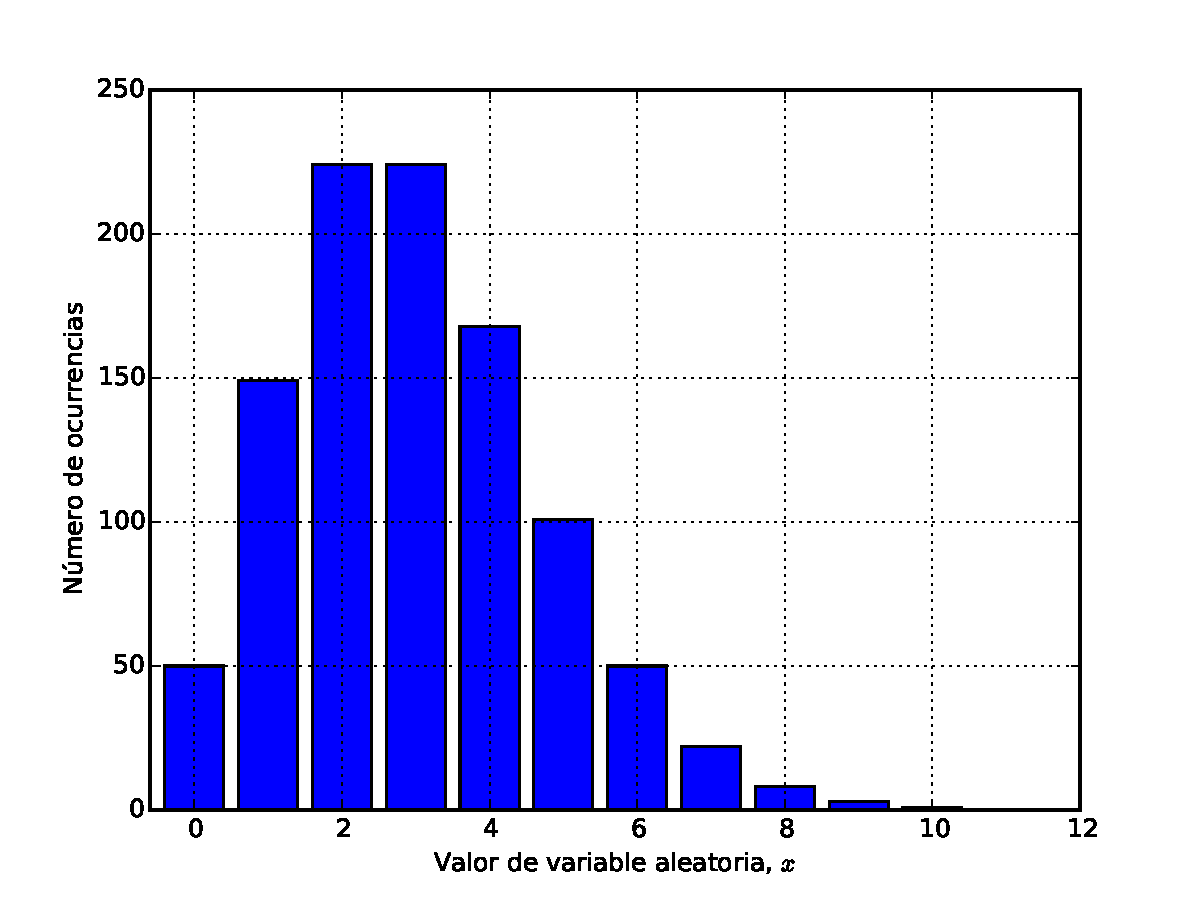
\includegraphics[width=9cm]{figs/fig-Poisson.pdf}
%\caption{n'umero de part'iculas $\alpha$ emitidas en un intervalo de tiempo dado. C'odigo Python en ap'endice \ref{app-Poisson}.}
%\end{center}
%\label{fig-Poisson}
%\end{figure}
\begin{figure}[h!]
\begin{center}
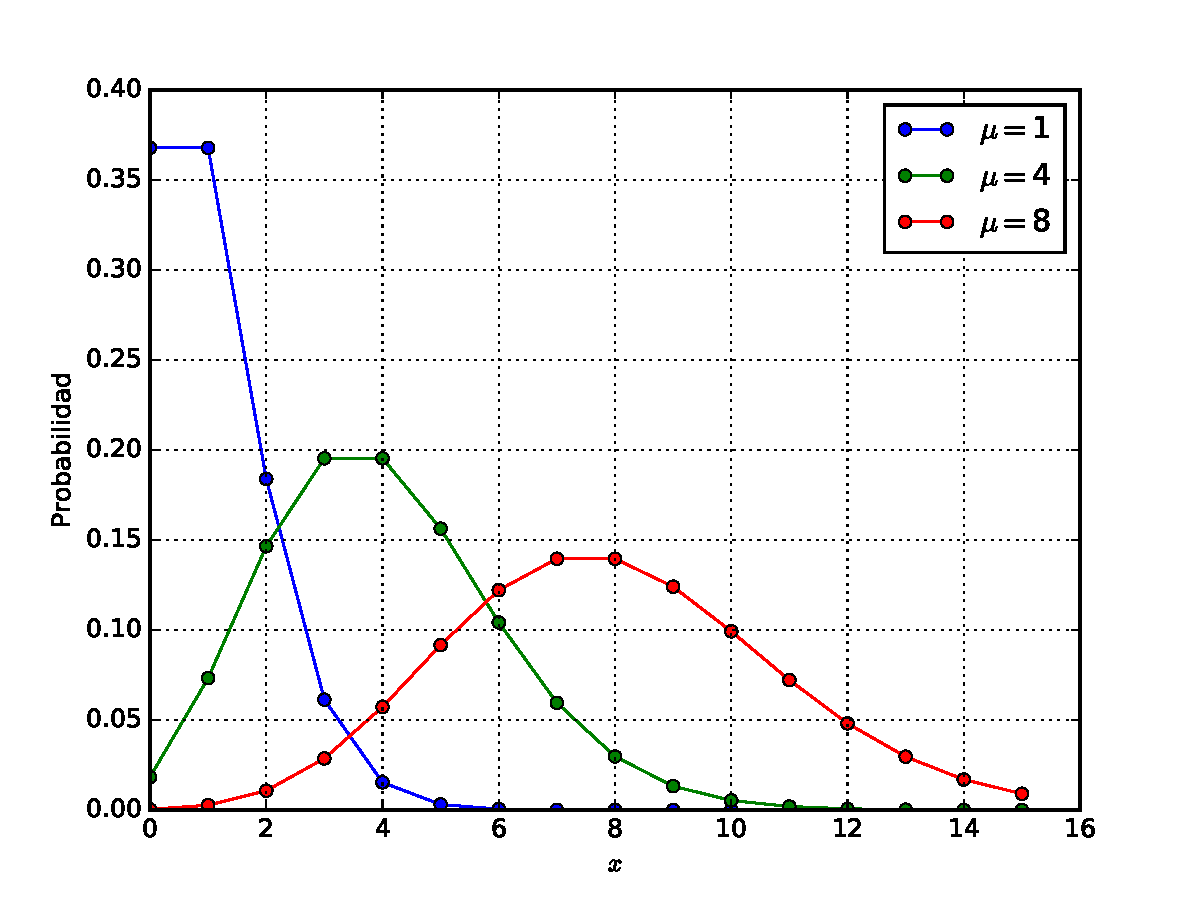
\includegraphics[width=9cm]{figs/fig-probabilidad-Poisson.pdf}
\caption{Funci'on probabilidad de Poisson. C'odigo Python \href{https://github.com/gfrubi/Lab/blob/master/python/fig-probabilidad-Poisson.py}{aqu\'i}.}
\end{center}
\label{fig-probabilidad-Poisson}
\end{figure}
\paragraph{Definici'on:} Sea $X$ una variable aleatoria que representa el n'umero de eventos aleatorios independientes que ocurren en un cierto intervalo (de tiempo, espacio, etc.). Se dice entonces que la variable aleatoria $X$ tiene una \textbf{distribuci'on de Poisson} si su  funci'on de probabilidad es dada por
\begin{equation}
P(x,\mu)=\frac{e^{-\mu}\mu^x}{x!}, \qquad x=0,1,2,3,\cdots,\quad \mu>0 .
\end{equation}
El par'ametro $\mu$ de la distribici'on es el \textbf{n'umero medio de sucesos esperados} (n'umero promedio de ocurrencias del evento en el intervalo de observaci'on, ya sea tiempo, distancia, etc.). Esta distribuci'on de probabilidad satisface las siguientes propiedades:
\begin{itemize}
\item Condici'on de normalizaci'on,
\begin{equation}
\sum_{x=0}^\infty P(x,\mu)=1.
\end{equation}
\item Valor medio,
\begin{equation}
\mu_{X}=\sum_{x=0}^\infty xP(x,\mu)=\mu.
\end{equation}
\item Varianza,
\begin{equation}
\sigma^2=\sum_{x=0}^\infty (x-\mu)^2P(x,\mu)=\mu,  
\end{equation}
\item Desviaci'on est'andar,
\begin{equation}
\sigma=\sqrt{\mu}.
\end{equation}
\end{itemize}

En general, la distribuci'on de probabilidad de Poisson es el modelo matem'atico que describe procesos en los que se satisfacen las siguientes propiedades:
Se dice que el proceso es de Poisson si satisface que, al dividirse el conteo en sub-intervalos suficientemente peque\~nos:
\begin{itemize}
\item La probabilidad de \textit{ocurrencia simult'anea} de dos eventos es nula.
\item Los eventos ocurren en forma \textit{independiente}.
\item La probabilidad de ocurrencia de un evento \textit{por intervalo} (de tiempo, o distancia, etc.) es constante. Equivalentemente, la probabilidad de ocurrencia de un evento \textit{es proporcional al intervalo} (de tiempo, o distancia, etc.) de observaci'on.
\end{itemize}

En el ejemplo de los decaimientos radiactivos, las condiciones listadas arriba parecen hip'otesis razonables, por lo que esperamos que este tipo de proceso pueda modelarse apropiadamente como un proceso de Poisson. En particular, si $\nu$ es el \textbf{n'umero medio de decaimientos por unidad de tiempo}\footnote{En Mec'anica Cu'antica es usual poder calcular la \textbf{probabilidad por unidad de tiempo}, $\dot{P}_{\rm dec}$, que un n'ucleo radiactivo decaiga. En este caso, $\nu={\cal N}\dot{P}_{\rm dec}$, donde $\cal N$ es el n'umero total de n'ucleos presentes en la muestra analizada.} de que se produzca un decaimiento en el material, entonces $\mu=\nu\Delta t$ es el n'umero medio de decaimientos esperados en el intervalo de tiempo $\Delta t$.

\paragraph{Ejemplo:} Se estima que cada a\~no se producen aproximadamente 13000 sismos de magnitud mayor que 4 en el mundo. Suponiendo que 'estos se distribuyen aleatoriamente en el a\~no y que son independientes, deber'iamos este proceso sea de Poisson. Estime la probabilidad de que se produzcan 5 sismos de estas caracter'isticas durante la misma hora. % mu = 13000/365 = 35.6 sismos/dia  = 1.48 sismos/hora, p(5,1.48)*100 = 1.35%

\subsection{Distribuci'on de probabilidad de una variable aleatoria continua: densidad de probabilidad}
Cuando la variable aleatoria puede tomar cualquier valor dentro de un cierto intervalo de n'umeros reales, diremos que la variable aleatoria es \textbf{continua}.

\paragraph{Definici'on:} Una funci'on $f_X(x)$ es una \textbf{funci'on de densidad de probabilidad} de la variable aleatoria continua X si para cualquier intervalo de n'umeros reales $[x_1,x_2]$:
\begin{enumerate}
\item $f_X(x)\geq 0$,
\item $\int_{-\infty}^\infty f_X(x)\,dx=1$,
\item $P(x_1\le X\le x_2)=\int_{x_1}^{x_2}f_X(u)\,du$.
\end{enumerate}

Esto permite interpretar $f_X(x)\,dx$ como la probabilidad de que la variable $X$ asuma un valor entre $x$ y $x+dx$. Es importate recordar que $f_X(x)$ no es directamente el valor de la probabilidad sino que es la ``probabilidad por unidad de intervalo de $x$". Esto se refleja tambi'en en las unidades de medida de $f_X(x)$:
\begin{equation}
[f_X]=\frac{[P]}{[\Delta x]}=\frac{1}{[x]}.
\end{equation}
As'i, por ejemplo, si la variable aleatoria $x$ representa una distancia, entonces $[x]=L$ y $[f_X]=L^{-1}$.


\paragraph{Definici'on:} La \textbf{funci'on distribuci'on acumulada} de una variable aleatoria continua $X$ es
\begin{equation}
F_X(x)=P(X\le x)=\int_{-\infty}^x f_X(u)\,du.
\end{equation}



\paragraph{Definici'on:} Si $X$ es una variable aleatoria continua con funci'on de densidad de probabilidad $f_X(x)$, $-\infty<x<\infty$, entonces la \textbf{media} de $X$, est'a definida por
\begin{equation}
\mu=\int_{-\infty}^\infty xf_X(x)\,dx.
\end{equation}
Adem'as, la \textbf{varianza} de $X$ es definida por 
\begin{equation}
\sigma_X^2=\int_{-\infty}^\infty (x-\mu)^2f_X(x)\,dx.
\end{equation}
La \textbf{desviaci'on est'andar} es entonces
\begin{equation}
\sigma_X=\sqrt{\sigma_X^2}=\sqrt{\int_{-\infty}^\infty (x-\mu)^2f_X(x)\,dx}.
\end{equation}


\begin{figure}[h!]
\begin{center}
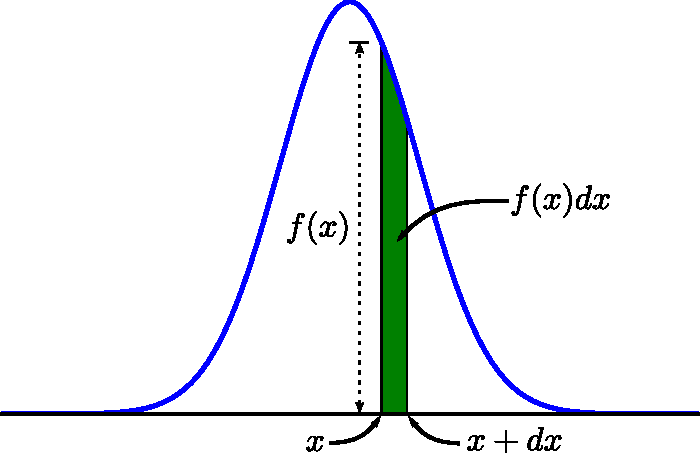
\includegraphics[width=8cm]{figs/fig-densidad-de-probabilidad.pdf}
\caption{Densidad de probabilidad.}
\end{center}
\label{fig-dens-prob}
\end{figure}
\subsection{Distribuci'on de Gauss o Normal}
	
%\paragraph{Ejemplo} 
%Al hacer estudios del poder de frenado (Stopping Power) lo que se desea describir es la p'erdida media de energ'ia de un has de part'iculas al viajar por el interior de un material. Supongamos que se hace incidir protones sobre una l'amina delgada de oro. Si graficamos la energ'ia de los protones dividida en intervalos de clase, luego que estos han atravesado la l'amina de oro, en el eje de las abscisas y el n'umero de protones correspondiente a cada intervalo en el eje de las ordenadas.

%\begin{figure}[h!]
%\begin{center}
%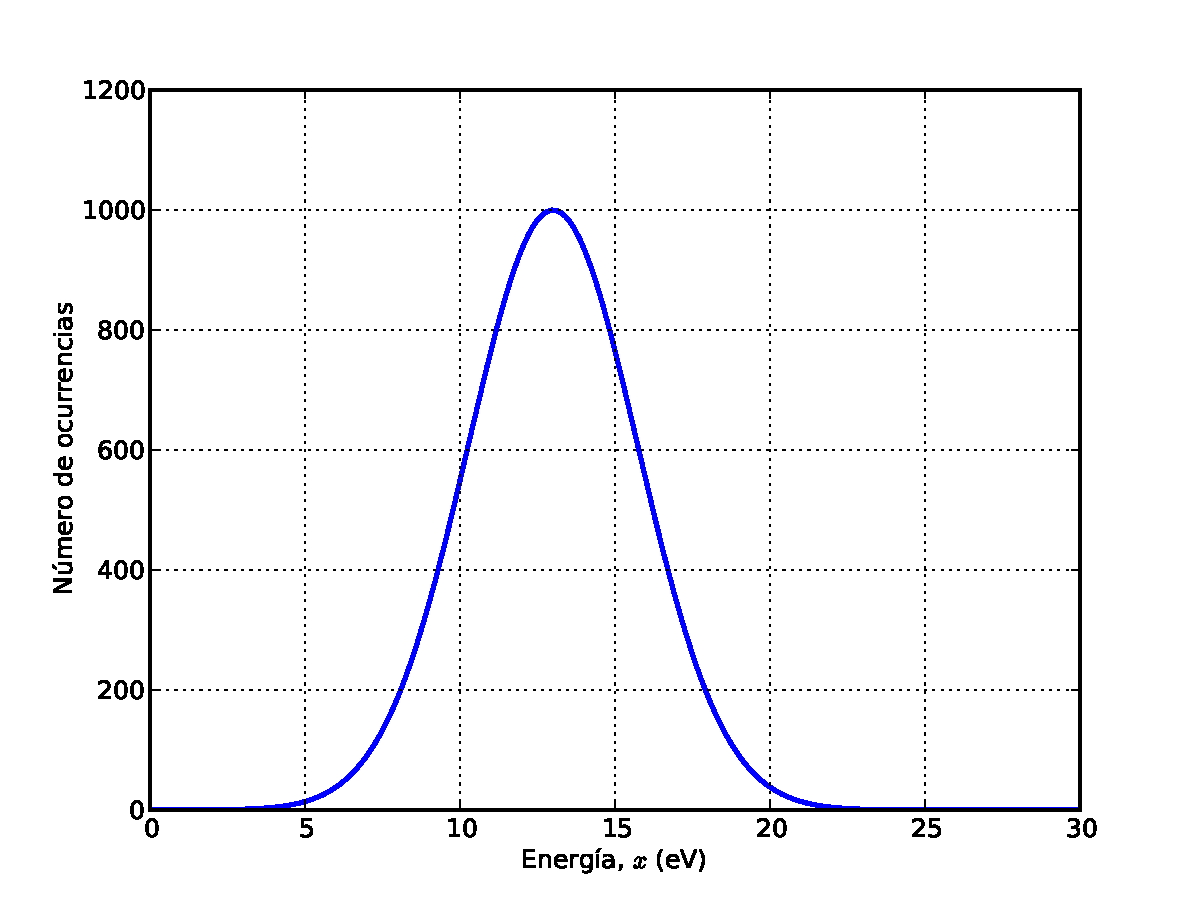
\includegraphics[width=9cm]{figs/fig-Gauss.pdf}
%\caption{P'erdida de energ'ia de protones luego de atravesar una l'amina de oro. C'odigo Python en ap'endice \ref{app-Gauss}.}
%\end{center}
%\label{fig-Gauss}
%\end{figure}

%	Retomando nuestros tres ejemplos de histogramas y normalizando cada uno de estos al n'umero total de eventos (si pensamos en t'erminos de una funci'on continua, seria normalizando al 'area de la curva)
%		


\begin{figure}[h!]
\begin{center}
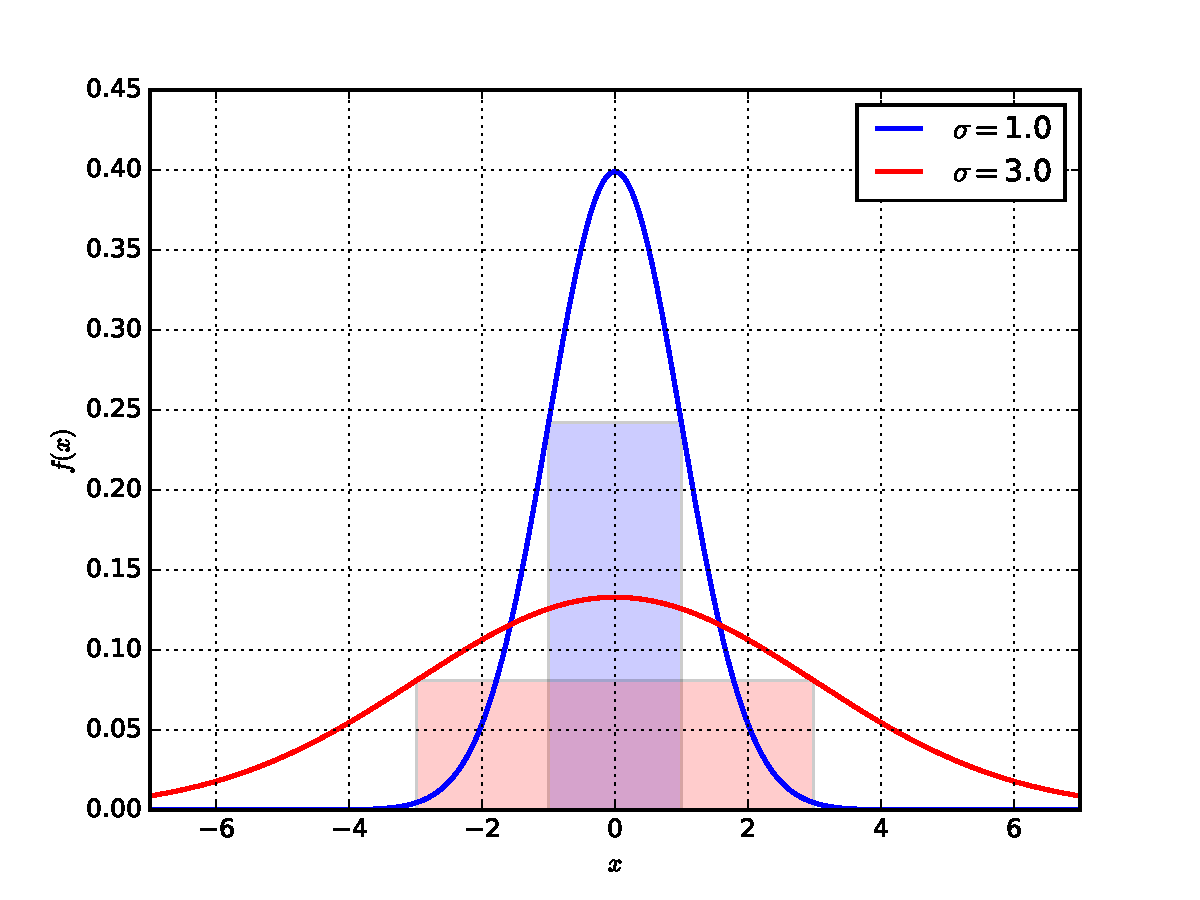
\includegraphics[width=9cm]{figs/fig-normal.pdf}
\caption{Distribuci'on normal.C'odigo Python \href{https://github.com/gfrubi/Lab/blob/master/python/fig-normal.py}{aqu\'i}.}
\end{center}
\label{fig-normal}
\end{figure}


\paragraph{Definici'on:} Se dice que una variable aleatoria $X$, se encuentra \textbf{normalmente distribuida} (Distribuci'on de Gauss) si su funci'on densidad de probabilidad est'a dada por:
\begin{equation}
f(x;\mu,\sigma)=\frac{1}{\sqrt{2\pi\sigma^2}}e^{-\frac{1}{2}\left(\frac{x-\mu}{\sigma}\right)^2}, \qquad -\infty<x<\infty,
\end{equation}
donde $-\infty<\mu<\infty$ y $\sigma>0$ denotan la media y la desviaci'on est'andar de $X$, respectivamente.  


\subsubsection{Propiedades}

Si $X$ es una variable aleatoria normal con valor medio $\bar{x}=\mu$ y varianza $\sigma_x^2=\sigma^2$, entonces la variable aleatoria
\begin{equation}
z=\frac{(x-\mu)}{\sigma}
\end{equation}
es una \textbf{variable aleatoria normal} con $\bar{z}=0$ y varianza $\sigma_z^2=1$. Esto es, $Z$ es una variable aleatoria normal est'andar.
La creaci'on de una variable aleatoria con esta transformaci'on se conoce como \textbf{estandarizaci'on}. La variable aleatoria $Z$ representa la diferencia de $X$ y su promedio, en unidades de desviaciones est'andar.

\paragraph{Utilidad de la estandariaci'on:}
Suponga que $X$ es una variable aleatoria con distribuci'on normal con media $\mu$ y varianza $\sigma^2$. Entonces,
\begin{equation}
P(X\leq x)=P\left(\frac{(X-\mu)}{\sigma} \leq \frac{(x-\mu)}{\sigma}\right)=P(Z\leq z),
\end{equation} 
donde
$Z$ es una variable aleatoria normal, y $z:=(x-\mu)/\sigma$ es el valor de $z$ obtenido a trav'es de la estandarizaci'on de $X$.

An'alogamente, es posible definir la \textbf{funci'on distribuci'on acumulada} de una variable aleatoria normal est'andar como
\begin{equation}
\Phi(z)=P(Z\leq z).
\end{equation} 

Los puntos de inflexi'on, la \textbf{media}, la \textbf{varianza} y la desviaci'on est'andar, usando la funci'on distribuci'on estandarizada, estar'ian dadas por
\begin{align}
f(x) = \frac{1}{\sqrt{2\pi\sigma^2}} e^{-\frac{1}{2}\left(\frac{x-\mu}{\sigma}\right)^2} =\frac{1}{\sqrt{2\pi\sigma^2}} e^{-\frac{1}{2}z^2},
\end{align}
%\begin{align}
%\frac{df(z)}{dz}&= \frac{-2z}{2\sqrt{2\pi\sigma^2}} e^{-z^2/2}=0 \\
%&\Rightarrow z=\frac{(x-\mu)}{\sigma}=0\\
%& x=\mu
%\end{align}
\begin{align}
\frac{d^2 f(z)}{dz^2}\stackrel{!}{=}0 \quad
\Rightarrow \quad  \frac{1}{\sqrt{2\pi\sigma^2}}e^{-z^2/2}  ( z^2 - 1 )=0 \quad 
\Rightarrow\quad z=\pm 1 \quad \Rightarrow\quad x=\mu \pm \sigma
\end{align}
\begin{align}
\bar{x} &= \frac{1}{\sqrt{2\pi\sigma^2}}\int_{-\infty}^\infty x e^{-\frac{1}{2}\left(\frac{x-\mu}{\sigma}\right)^2}dx \\
&= \frac{1}{\sqrt{2\pi}} \int_{-\infty}^\infty (\mu+\sigma z) e^{-z^2/2}dz \\
&= \frac{\mu}{\sqrt{2\pi}} \int_{-\infty}^\infty e^{-z^2/2}dz+0 \\
&= \frac{\mu}{\sqrt{2\pi}}(\sqrt{2\pi})\\
&= \mu
\end{align}
\begin{align}
\sigma_X^2 &= \frac{1}{\sqrt{2\pi\sigma^2}}\int_{-\infty}^\infty (x-\mu)^2 e^{-\frac{1}{2}\left(\frac{x-\mu}{\sigma}\right)^2}dx \\
&= \frac{1}{\sqrt{2\pi}}\int_{-\infty}^\infty (\sigma z)^2 e^{-z^2/2}dz \\
&= -\frac{\sigma^2}{\sqrt{2\pi}}\int_{-\infty}^\infty z\frac{d}{dz}\left(e^{-z^2/2}\right)dz \\
&=-\frac{\sigma^2}{\sqrt{2\pi}}\left[\left.ze^{-z^2/2}\right|_{-\infty}^\infty-\int_{-\infty}^\infty e^{-z^2/2} dz\right] \\
&=-\frac{\sigma^2}{\sqrt{2\pi}}\left[0-\sqrt{2\pi}\right] \\
&= \sigma^2.
\end{align}

\begin{align}
\sigma_x=\sqrt{\sigma_x^2}=\sigma,
\end{align}
respectivamente.


